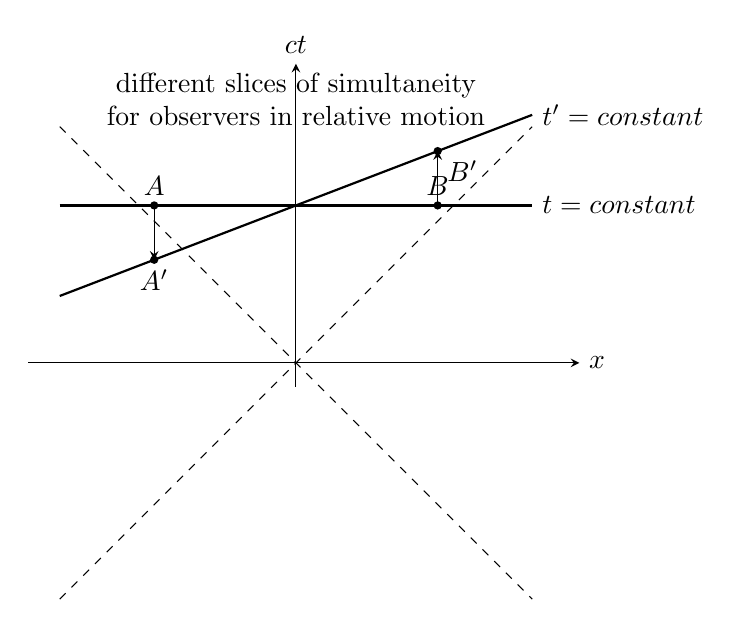
\begin{tikzpicture}[x=1cm,y=1cm,>=stealth]
    \draw[->] (-3.4,0) -- (3.6,0) node[right] {\(x\)};
    \draw[->] (0,-0.3) -- (0,3.8) node[above] {\(ct\)};

    \draw[dashed] (-3,-3) -- (3,3);
    \draw[dashed] (-3,3) -- (3,-3);

    % laboratory simultaneity
    \draw[thick] (-3,2.0) -- (3,2.0) node[right] {\(t=\text{constant}\)};
    \fill (-1.8,2.0) circle (1.5pt) node[above] {\(A\)};
    \fill (1.8,2.0) circle (1.5pt) node[above] {\(B\)};

    % moving-frame simultaneity, ct' constant: ct - beta x = const
    \draw[thick] (-3,0.85) -- (3,3.15) node[right] {\(t'=\text{constant}\)};
    \fill (-1.8,1.31) circle (1.5pt) node[below] {\(A'\)};
    \fill (1.8,2.69) circle (1.5pt) node[below right] {\(B'\)};

    \draw[->] (-1.8,2.0) -- (-1.8,1.31);
    \draw[->] (1.8,2.0) -- (1.8,2.69);
    \node[align=center] at (0,3.35) {different slices of simultaneity\\for observers in relative motion};
\end{tikzpicture}
